\documentclass[a4paper,11pt,oneside,oldfontcommands]{memoir}
\usepackage{ecis2015}
\usepackage{datetime}    			% sourced from; http://ftp.snt.utwente.nl/pub/software/tex/macros/latex/contrib/datetime/
\usepackage{longtable}

%\usepackage{amssymb, setspace, rotating, titlesec, adjustbox, array, threeparttable}
\usepackage{amssymb, setspace, rotating, titlesec, adjustbox, array, threeparttable}
									% is all of this necessary?? 
%%%%%%%%%%%%%%%%%									
%% Fonts, fonts, fonts, notably for math
\usepackage{xfrac}					% tbv slanted fractions: \sfrac{}{}
\usepackage{pifont}

\RequirePackage[utf8]{inputenc}		% NOT required when using xetex as opposed to pdftex

\usepackage[T1]{fontenc}

\usepackage{amsmath}				% <amsmath> needs to be loaded before ntheorem (section 3.2.1, ftp://ftp.dante.de/pub/tex/macros/latex/contrib/ntheorem/ntheorem.pdf) 
\usepackage[mathcal]{euscript}		% tbv de gecalligrafeerde mathcal{O} en W(orld) en (M)odel etc. Refer to http://texdoc.net/texmf-dist/doc/fonts/amsfonts/euscript.pdf
									% Note that, in fact, eucal and euscript are identical, except that they use different commands (\mathcal and \mathscr). By using euscript 
									% we only provide \mathscr{} and leave \mathcal{} from amsmath unchanged
\usepackage{pgothic}				% Used for modern gothic that has a readible S
\DeclareMathAlphabet{\mathgoth}{T1}{pgoth}{m}{n}	% Declaring the pgothic family as math alphabet
%\usepackage{addfont}				% This would be an alternative for the readible S font, but not working
%\addfont[1.25]{OT1}{hge}{\hge}
%\DeclareMathAlphabet{\mathgoth}{OT1}{hge}{m}{n}	% Declaring the hge family as math alphabet

\usepackage{lmodern}				% necessary in combination with CMcal-font from mathcal/euscript to generate the font that is necessary for the Interpretation function \CMcal{I}
\usepackage{amssymb}				% necessary for (at least) the \mathbb font
\usepackage{mathrsfs}				% necessary for (at least) the \mathpzc font
\DeclareMathAlphabet{\mathpzc}{OT1}{pzc}{l}{it}		% Declaring the pzc font as math alphabet (not used, yet)


\usepackage[normalem]{ulem}			% tbv strikout text: \sout{deze tekst is strikeout}
\usepackage{siunitx}				% Necessary??

%\usepackage{fourier} 				% Assuming that you are using venturis for text, Hirwen Harendal, who designed the collection, advises that the best choice for mathematics is
									%	fourier and the second best is mathdesign. Fourier sets text and math fonts.
\usepackage{venturis2}				% Ik wil het font Venturis ADF No2 toepassen als Normalfont
									% 	Ik kan ook overwegen Obyknovennaya Novaya te gebruiken, ook fraai. Gevonden op http://www.tug.dk/FontCatalogue/venturisadfno2/

%% End of Fonts
%%%%%%%%%%%%%%%

\usepackage{xcolor}
%%\usepackage{MnSymbol}				% Levert foutmelding: Too many math alphabets used in version normal. 
\usepackage[xindy,toc]{glossaries}	%%%% The glossaries environment. Refer to: http://en.wikibooks.org/wiki/LaTeX/Glossary
%%%\usepackage{pst-plot}				%%%% The ps trick environment. Zie ook: http://tug.org/PSTricks/main.cgi?file=examples REQUIRES --latex-engine=xelatex

%% Theorems
\usepackage[ntheorem]{empheq}
\usepackage[thmmarks]{ntheorem}		% Easier handling of theorem-like environments. refer to ftp://ftp.dante.de/pub/tex/macros/latex/contrib/ntheorem/ntheorem.pdf

\usepackage{datetime}    			 % sourced from; http://ftp.snt.utwente.nl/pub/software/tex/macros/latex/contrib/datetime/
\usepackage{mdframed}

%% Figures and table placement		% Sourced from http://tug.ctan.org/tex-archive/info/epslatex/english/epslatex.pdf page 55
\usepackage{flafter}				% Ensure that the figures/tables appear after its figure/table environment definition in the text

\makeatletter						% Change the default figure / table placement from [tbp] to [htbp]; this is useful since mmd prevents us to insert the placement parameters ourselves
\def\fps@figure{htbp}
\def\fps@table{htbp}
\makeatother

\usepackage[section]{placeins}		% Since it is often desirable to keep floats in the section in which they were issued, insert a \FloatBarrier command before each section.

%% Drawings by LaTeXDraw
%\usepackage{auto-pst-pdf}			% To use pstricks in pdflatex: https://tex.stackexchange.com/questions/8413/how-to-use-pstricks-in-pdflatex
%\usepackage[pdf,usenames,dvipsnames]{pstricks}
%\usepackage{epsfig}
%\usepackage{pst-grad} % For gradients
% \usepackage{pst-plot} % For axes
%\usepackage[space]{grffile} % For spaces in paths
%\usepackage{etoolbox} % For spaces in paths
%\makeatletter % For spaces in paths
%\patchcmd\Gread@eps{\@inputcheck#1 }{\@inputcheck"#1"\relax}{}{}
%\makeatother


%% Logical proofs
\usepackage{lplfitch}				% sourced from https://github.com/rzach/lplfitch
%									% documentation from http://ftp.snt.utwente.nl/pub/software/tex/macros/latex/contrib/lplfitch/lplfitch.pdf
%\usepackage{fitch}					% The fitch package is more simple to use than lplfitch

%% Lists
%\usepackage[ampersand]{easylist}	% The easylist environment
\usepackage{enumitem}				% List manipulation package

%% Grammars
\usepackage[epsilon]{backnaur}		% For creation of BNF grammars. Refer to http://ctan.cs.uu.nl/macros/latex/contrib/backnaur/backnaur.pdf 

%% Lorem ipsum generated text
\usepackage{blindtext}

%% ToDo's							% Creating proper todo bubbles adjacent to text. Refer to http://ctan.triasinformatica.nl/macros/latex/contrib/todonotes/todonotes.pdf
\usepackage[textsize=tiny,colorinlistoftodos]{todonotes}	

%% Cross-referencing				% Allow the format of cross-references to be determined automatically according to the “type” of cross-reference (equation, section, etc.) and the context in which the cross-reference is used.
%\usepackage{varioref}				% sourced from http://texdoc.net/texmf-dist/doc/latex/tools/varioref.pdf
\usepackage{hyperref}				% If we want to use hyperref, sometime in the future for some reason, it should be defined in between of varioref and cleveref
\usepackage{cleveref}				% sourced from http://tug.ctan.org/macros/latex/contrib/cleveref/cleveref.pdf Makes varioref clever, and reuses its work to improve its own workings. 
									% The cleveref package must be loaded after all other packages that don’t specifically support it.
									% Therefore, to be safe, we declare it as last in the document's preamble.
									% Also note that all \newtheorem definitions must be placed after the cleveref package is loaded.

%% Table stuff						% sourced from: https://tex.stackexchange.com/questions/33510/how-do-i-create-the-headings-for-this-multirow-multicolum-table
\usepackage{graphicx}
\usepackage{multirow}
\usepackage{booktabs}

%%% About this LaTeX template: %%%%%%%%%%%%%%%%%%%%%%%%%%%%%%%%%%%%%%%%%%%%%%%
%
% This template should work with any (reasonably recent) full
% installation of TeXLive or MikTeX. The "ecis2015" package loads a
% number of other packages, so if some package is missing, please
% install it using the package manager of your TeX distribution. In
% particular, if the "tikz" package is missing, you may have to install
% "pgf" or simply remove our example graphics (see figure example
% below).
%
% The file "ecis2015.sty" should be placed somewhere in your TeX Path
% (or simply in the same folder as your document).
%
% Please use PDFLaTeX to compile your document.
%
% You need not escape special characters or Umlauts like é ä ö ü ß (in 
% fact, you shouldn't), as this source is inputenc'd in UTF-8.
%
% Note for BibTeX users: We use BibLaTeX for formatting, so we use Biber
% as a sorting backend (default). 
% If you still need to use the old BibTeX program, please change the 
% BibLaTeX backend in the package file ("ecis2015.sty").
%
%%%%%%%%%%%%%%%%%%%%%%%%%%%%%%%%%%%%%%%%%%%%%%%%%%%%%%%%%%%%%%%%%%%%%%%%%%%%%%


%%% ------- mijn configs: --------- %%%
%
%% test stuff

% Redefining the paragraph level into a case - see https://tex.stackexchange.com/questions/129208/numbering-paragraphs-in-latex
\newcounter{para}
\renewcommand\paragraph[1]{%
  {\par\refstepcounter{para}\textbf{Case \thepara:\space#1\space}\label{#1}}
}

%% end test stuff


%%
%% Defining new theorem and -styles
% Its documentation can be found at ftp://ftp.dante.de/pub/tex/macros/latex/contrib/ntheorem/ntheorem.pdf
%\RequirePackage[thref, thmmarks, amsmath]{ntheorem}		% Use new theorems package as opposed to amsth, include <amsmath>-emulation by including it as an option

% Allow to repeat a theorem number to, e.g., continue with a theorem such as an example, or to add something to an existing theorem
% THIS UNFORTUNATELY DOES NOT WORK, producing a <Undefined control sequence \n <argument> \rep@title \n l.38 \newtheorem*{rep@theorem}{\rep@title}>-error
%\makeatletter
%\newtheorem*{rep@theorem}{\rep@title}
%\newcommand{\newreptheorem}[2]{%
%\newenvironment{rep#1}[1]{%
% \def\rep@title{#2 \ref{##1}}%
% \begin{rep@theorem}}%
% {\end{rep@theorem}}}
%\makeatother
	
%%%%% Theorems Definitions %%%%%%
\theoremstyle{definition}
\theoremstyle{break}		% The header for all theorems are followed by a newline
% Examples 					-- are numbered by chapter, and carry an asterisk as closing symbol
\theoremsymbol{\ensuremath{_\Box}}
\newtheorem{mmexmp}{Example}[chapter]
%\newreptheorem{mmexmp}{Example (cont'd)}
% Theses   					-- have continuous numbering scheme, and still close with the asterisk
\newtheorem{Thesis}{Thesis}
% Research Questions 		-- are enclosed with horizontal lines, and probably (?) close with the asterisk
\theoremprework{\hrule}
\theorempostwork{\hrule}
\newtheorem{mmthrq}{Research Question}
% Assumption				-- are numbered by chapter, and carry an asterisk as closing symbol
\newtheorem{mmasmptn}{Assumption}[chapter]
% Definitions & theorems	-- are numbered by chapter, and carry a black square as closing symbol
\theoremsymbol{\ensuremath{_\blacksquare}}
\newtheorem{mmdef}{Definition}[chapter]
\newtheorem{mmtrm}{Theorem}[chapter]
% Design Principles, proofs	-- are numbered by chapter, and carry an open diamond as closing symbol
\theoremsymbol{\ensuremath{_\diamond}}
\newtheorem{mmdp}{Design Principle}[chapter]
\newtheorem{mmprf}{Proof}[chapter]
% Remarks to tables, figures, whatever -- restart numbering at sections, no closing symbol
\theoremsymbol{}			% no symbol
\theorembodyfont{\upshape}	% no slanted or italics
\newtheorem{mmrmk}{Remark}[subsection]	% theorem counter resets every \subsection
\renewcommand{\themmrmk}{(\arabic{mmrmk})}	% Remove subsection from theorem counter representation

% Names of the theorems
\crefname{mmexmp}{Example}{Examples}
\crefname{Thesis}{Thesis}{Theses}
\crefname{mmthrq}{Research Question}{Research Questions}
\crefname{mmdef}{Definition}{Definitions}
\crefname{mmtrm}{Theorem}{Theorems}
\crefname{mmprf}{Proof}{Proofs}
\crefname{mmdp}{Design Principle}{Design Principles}
\crefname{mmasmptn}{Assumption}{Assumptions}
\crefname{mmrmk}{Remark}{Remarks}
\crefname{chapter}{Chapter}{Chapters}
\crefname{section}{Section}{Sections}
\crefname{figure}{Figure}{Figures}
\crefname{table}{Table}{Tables}
\crefname{equation}{Eq.}{Eqs.}

% Definition of List of Theorems (\listtheorems{<name>})
\theoremlisttype{opt}

%%%%%%%% End Theorems definitions

% Equations				-- are numbered by chapter
\numberwithin{equation}{chapter}
% Figures				-- are numbered by chapter
\numberwithin{figure}{chapter}

% package backnaur: modify the production operator
\renewcommand*{\bnfpo}{\textnormal{::=}}

% some more mnemonic terms 
\newcommand*\OK{\ding{51}}		% for the check-marks
\newcommand*\ntsa{\ensuremath{\varnothing}}	% no transcription allowed

% Create a typical column header, the content of which is rotated
\newcolumntype{R}[2]{%
 >{\adjustbox{angle=#1,lap=\width-(#2)}\bgroup}%
 l%
 <{\egroup}%
}
\newcommand*\rot{\multicolumn{1}{R{60}{1em}}}% no optional argument here, please!

% Create a command for words in a box. Refer to http://tex.stackexchange.com/questions/86569/creating-uniformly-sized-boxes-around-text, and 
%                                      for the colors to http://tex.stackexchange.com/questions/136742/changing-background-color-of-text-in-latex
\newcommand{\mywordbox}[1]{%
  {% open a group for a local setting
   \setlength{\fboxsep}{-2\fboxrule}% the rule will be inside the box boundary
   \hspace{1pt}\fcolorbox{gray!20}{blue!5}{\hspace{2pt}\strut\textbf{#1}\hspace{2pt}}\hspace{1pt}% print the box, with some padding at the left and right
%   \fbox{\hspace{2pt}\strut\text{#1}\hspace{2pt}}% print the box, with some padding at the left and right
%   \fbox{\hspace{2pt}\strut#1\hspace{2pt}}% print the box, with some padding at the left and right
  }% close the group
}


%%% Enter Document Info here: %%%%%%%%%%%%%%%%%%%%%%%%%%%%%%%%%%%%%%%%%%%%%%%%
%%%datetime package config %%%
\renewcommand{\dateseparator}{-}
%\renewcommand{\timeseparator}{}
\settimeformat{hhmmsstime}  

\maintitle{Consolidating semantic interoperability in software architectures} % ← Don't use UPPERCASE here, we do that automatically.
\subtitle{Access-and-play semantic interoperability in contemporary architectural
paradigms}
\shorttitle{} % ← This goes into the header.
\category{} % 

\date{\today}


\authors{% Separate authors by a "\par" or blank line.
Paul Brandt,\\
Eindhoven University of Technology; Netherlands Organization of Applied
Scientific Research TNO, Den Haag, The Netherlands, 

\par
Eric Grandry,\\
Luxembourg Institute of Science and Technology, Esch-sur-Alzette,
Luxembourg, 

\par
Twan Basten,\\
Eindhoven University of Technology, Eindhoven, The Netherlands, 

\par
}
\shortauthors{Paul Brandt -- } % ← This goes into the header. 

%%% BibTeX: %%%%%%%%%%%%%%%%%%%%%%%%%%%%%%%%%%%%%%%%%%%%%%%%%%%%%%%%%%%%%%%%%%

\addbibresource{src/bib/CitedByMe-2018\_archSIOp.bib} % ← Your .bib file, if you're using BibTeX

%%%%%%%%%%%%%%%%%%%%%%%%%%%%%%%%%%%%%%%%%%%%%%%%%%%%%%%%%%%%%%%%%%%%%%%%%%%%%%

%%% Glossaries: %%%%%%%%%%%%%%%%%%%%%%%%%%%%%%%%%%%%%%%%%%%%%%%%%%%%%%%%%%%%%%

%%%%%%%%%%%%%%%%%%%%%%%%%%%%%%%%%%%%%%%%%%%%%%%%%%%%%%%%%%%%%%%%%%%%%%%%%%%%%%

\begin{document}
% Set the properties of the easylist

%\pagebreak

% --- Abstract --- --- --- --- ---
\begin{abstract}
\emph{Background:} Access-and-Play SIOp is the next glass ceiling in
{[}interoperability/IT-based business collaboration{]}. We can think of
two approaches to break through the ceiling, i.e., using either strong
AI (a system that can \emph{think} and has a \emph{mind}, in the
philosophical definition of the term) or weak AI (a system that can only
\emph{act} like it thinks and has a mind (Searle 1980)). Strong AI is
not yet available, while weak AI, despite its current applications in
Semantic Web or ontologies, has not yet been embedded in contemporary
software architectural paradigms. Current approaches towards SIOp can be
considered accepted folklore.

\emph{Objective:} The objective of this study is to identify and define
the (weak AI based) fundamental guidance towards access-and-play
semantic interoperability in contemporary architectural paradigms.

\emph{Method:} Our approach is based on the discipline of semiotics.
After identifying semiotic shortcomings in MDA and view-based
architectural paradigms and their subsequent definition as missing
concerns, we develop the necessary guiding architectural principles. We
finally consolidate their fundamentals as an ISO-42010 Architecture
Viewpoint to disclose them for the various architectural paradigms.
{[}We evaluate these principles by designing a reference architecture
and proof its use in SIOp between two software agents.{]}

\emph{Results:} The semiotic approach/discipline demonstrates/proves
semantics in software to be the result of a reciprocity between data and
the software code that operates on them. The major shortcomings in
architectural paradigms to account for semantic interoperability are
their negligence of semiotic fundamentals and, particularly, the absence
of an explicit ontological commitment that stands at the root of
semantics. Therefore, the concern about a semantic loose coupling should
be added to the architectural paradigms. The supporting principles are
(i) semantic transparency, (ii) semantic separation of concerns, and
(iii) explicit computational semantics. In view-based architectures
their consolidation implies a new semantic view, while the MDA paradigm
requires an ontological commitment on M3. Both paradigms need to include
a semantic alignment processing mediation capability.

\emph{Conclusions:} Access-and-play SIOp can be achieved when
considering semiotic fundamentals and adding loosely coupled formal
semantics to contemporary architectural paradigms.\\
\end{abstract}


% --- Keywords --- --- --- --- ---



%\pagebreak
% --- table of contents --- --- --- --- ---
%
% add table of contents to pdf bookmarks


% add list of todo's that are outstanding for this text


% --- main matter --- --- --- --- ---

\hypertarget{introduction}{%
\chapter{Introduction}\label{introduction}}

Never before, data were so ubiquitous, and managed access to external
data was so easy. Because current ICT is unable to \emph{use} all that
same external, non-native data as access-and-play service, agility in
business collaboration is hampered in all domains. For instance,
consider the following (allegedly real) example of an interoperability
failure.

\begin{quote}
A German steel producer upgraded its industrial process robot. Since the
majority of the steel production process is dependent on time, from a
security point of view the decision was made to not rely on their own
internal clocks but to use the German \emph{Braunschweig Funkuhr} time
radio signal as source for the exact time instead. At the end of April
1993, when Germany went on summer time, the computer clock of the steel
producer went from 1:59 AM to 3:00 AM in one minute. This resulted in a
production line allowing molten ingots to cool for one hour less than
normal. When the process controller thought the cooling time had
expired, his actions splattered still-molten steel, damaging part of the
facility.\footnote{Source:
  http://catless.ncl.ac.uk/Risks/14.57.html\#subj1, accessed May 20,
  2018}
\end{quote}

In this simple example a tiny difference in the meaning of \texttt{time}
between the steel producer and the national time provider hampered
interoperability to the extend of damaging the steel facility. This tiny
difference rooted in the assumption by the steel producer that
\texttt{time} expressed a continuous scale whilst for the Braunschweig
Funkuhr, \texttt{time} denoted instant clock time for that time zone and
therefore represented a non-continuous scale. In order to achieve that
both collaborators, here the Braunschweig Funkuhr and the steel
producer, can actually \emph{use} their peers data, the need exists to
design and implement wrappers that remove any inconsistency between the
variations that may occur in terms, structures, dimensions and what have
you. Many such variations exist, leading to a range of failures in
so-called \emph{semantic interoperability} (SIOp) and Section/Appendix
\#\# provides for a short overview of SIOp-faults. Unfortunately, it is
fundamentally impossible to automate the production of wrappers, because
we need a genuine \emph{understanding} upfront, which computers still
cannot do.

The most disconcerting consequences of a lack of (automated) SIOp are
time-to-deliver, flat interoperability failures, and even seemingly
correct but quite invalid data analysis probably leading to devastating
system behaviour. Current SIOp implementations are essentially based on
the (time-consuming) process of establishing a (local) convention on the
semantics of the terms that are exchanged during collaboration,
requiring custom solutions and collaboration-dependent software
adaptations. Such conventions can be considered a semantic monolith,
which makes dealing with data outside the monolith impossible, unless
again a time consuming (months) semantic adoption process is applied.
Moreover, these semantic conventions consider semantic heterogeneity as
a bug instead of a feature necessary to achieve semantic accuracy. But
still, this conventions-based approach towards SIOp is accepted folklore
in ICT. In view of the large uptake of the Internet, the Internet of
Things (IoT), cloud computing and big data, and in view of economical
pressure to intensify enterprise collaboration, we consider this
approach ``too little, too late''.

In comparison, scalability was a big architectural concern in the past,
requiring custom solutions as well. In response to this concern,
scalability was standardised in the form of architectural patterns, and
finally totally embedded and hidden into the infrastructure. Similarly,
SIOp can be considered the architectural concern of this decade, and we
first need to provide a standardised solution pattern to address
semantic concerns, before we can embed it in a technological
infrastructure so that SIOp becomes transparent to the developer. Where
scalability resulted in a huge increase in performance-demanding
applications against a fraction of the original costs and effort,
business agility will emerge once the semantic monolith is removed and
semantic services exist at the infrastructural level. Then SIOp becomes
an access-and-play operation that achieves SIOp in due time with data
not anticipated for during software design, at any point in their life
cycle. Metaphorically speaking, we consider SIOp as a \emph{bridge}
overarching a (semantic) gap: with \emph{bridgeheads} on each side of
the gap, with a \emph{spanning} resting on them to structurally support
the bridge and its traffic, and with a \emph{roadway} enabling the
crossing of the traffic. Finally, architectural \emph{principles}
provide the necessary guidance to the architect for the various design
decisions that effectively result in a particular bridge over a
particular (semantic) gap. Our contributions to consolidating semantic
interoperability in software architectures are fivefold, and represented
as architectural principles and concerns, as follows:

\begin{itemize}
\tightlist
\item
  \emph{Principles}: We base SIOp on establishing loose-coupling at the
  semantic level by introducing principles on semantic separation of
  concerns and semantic transparency (Section \ref{siop-principles}),
  and show how these principles can be operationalised;
\item
  \emph{Semantic concerns (bridgehead)}: Abstracting semantics from a
  tacit software implication into a tangible, computational and distinct
  artifact provides us with the potential to connect to it and to make
  comparisons with the semantic artifact of the peer software agent.
  Based on the discipline of semiotics, we explain the shortcomings of
  the current approach towards software semantics that rely on
  information models and information views. Instead, we provide for a
  fundamental notion on the application of ontologies {[}and ontological
  commitment{]} to remedy current semantic shortcomings, and we show
  {[}its/their{]} proper position in the total architecture (Section
  \ref{bridgehead-semantics});
\item
  \emph{Weak AI concerns (spanning)}: Since ``strong AI'' does not yet
  exist, SIOp remains in demand of human intervention in order to
  reconcile the semantic differences between collaborating software
  agents. However, human intervention is time consuming. We reduce the
  necessary human intervention to complement weak AI to a task that
  suffices to achieve SIOp, viz. authoring semantic alignments only
  (Section \ref{spanning-alignments});
\item
  \emph{Mediation concerns (roadway)}: We provide for a prototypical
  implementation of a mediator as the necessary component to
  automatically translate data when transferred between the
  collaborating software agents (Section \ref{roadway-mediation});
\item
  \emph{ISO42010 Architecture Viewpoint}: We formulate the architectural
  consequences of the above concerns as a specific SIOp Viewpoint in
  order to consolidate SIOp for contemporary architectural paradigms
  (Section \ref{architectural-viewpoint-on-siop});
\end{itemize}

Based on these contributions we {[}argue/defend{]} that access-and-play
SIOp can be embedded and hidden in infrastructural services when
considering semiotic fundamentals and adding loosely coupled formal
semantics to contemporary architectural paradigms. To that end, we first
describe the semiotic fundamentals in
\cref{the-semiotic-and-philosophical-foundations-of-semantics}.

\hypertarget{the-semiotic-and-philosophical-foundations-of-semantics}{%
\chapter{The semiotic and philosophical foundations of
semantics}\label{the-semiotic-and-philosophical-foundations-of-semantics}}

\hypertarget{semiotics}{%
\section{Semiotics}\label{semiotics}}

The discipline of semiotics is the study of signs, reality and meaning.
The meaning of a \emph{token} (text, graphics, sound) ultimately relates
to what it denotes in reality (the \emph{entity}), whilst this relation
cannot be deferred from the shape, structure or other characteristics of
the token itself due to its total arbitrariness. In the early 1900s, De
Saussure used a dyadic model that stressed that the token and the entity
in reality were as inseparable as the two sides of a piece of paper
(Saussure 1959). This piece of paper he called the
\textbf{\emph{semiotic sign}}, denoting the whole. This
`self-containment of the sign' remains one of the major principles of
semiotics. Constructing the semiotic sign from its distinct parts is
called \textbf{\emph{semeiosis}}. The token, in combination with their
ability for semeiosis, provides humans with the tool to converse with
each other. The tokens provide humans with a vocabulary, the semeiosis
makes them understand about what entities they talk about. Semantics,
then, emerges as a result of the semeiosis that connects the distinct
parts of the inseparable semiotic sign.

Sanders Peirce (in: Sowa 2000) developed another model to further
investigate the semeiosis part of semantics. He built a triadic model of
the semiotic sign, including a representamen (the token) and object (the
entity), and introduced the \emph{interpretant} which expresses the
mental and, hence, individual sense making. This triadic model of the
semiotic sign was coined by Peirce as the \emph{semiotic triangle}
(ibid.), depicted in \cref{fig:semiotic-triangles}(a), and subsequently
used and modified by Ullmann (Ullmann 1962), Ogden and Richards (Ogden
and Richards 1989), and many others. We introduce our modifications, as
depicted in \cref{fig:semiotic-triangles}(b), which mainly focus on
naming conventions in IT architectures, as follows.

\begin{figure}
\hypertarget{fig:semiotic-triangles}{%
\centering
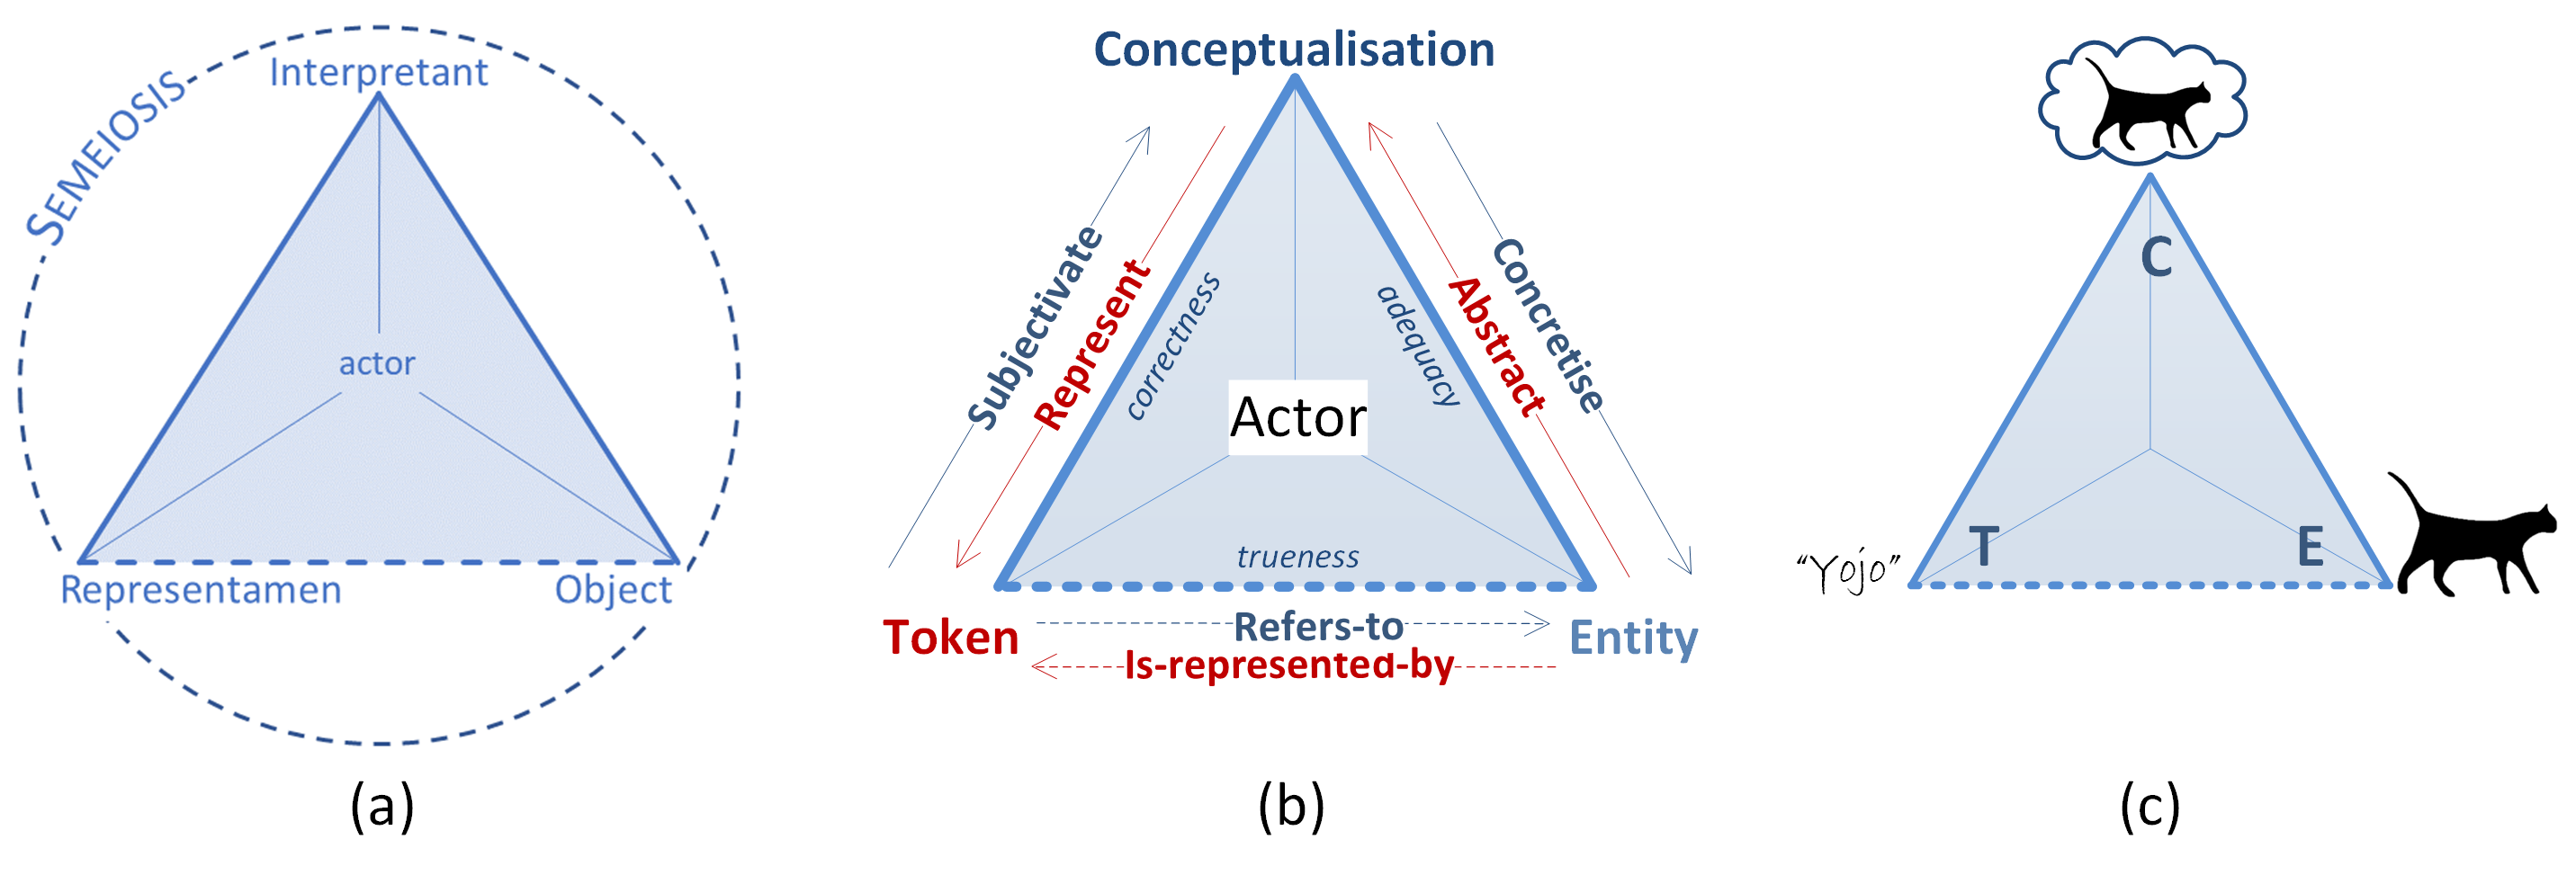
\includegraphics[width=6.25in,height=2.08333in]{./tex2pdf.9980/1d52e69a092840696e68cfe7d8fce2e0b93e3240.png}
\caption{The triadic model of the semiotic sign, according to Peirce
(a), and modified by us (b). Example (c) shows the concept of a cat
named ``Yojo''}\label{fig:semiotic-triangles}
}
\end{figure}

Where Peirce denotes the \emph{object}, we prefer the use of
\emph{entity} due to the ambiguous nature of the former in IT modelling
and architectures. We consider an entity to stand for a thing or an
event, but also a category of entities, a relation between entities and
a property of an entity. We will refer to the \emph{interpretant}
component as the \emph{conceptualisation}, to underline the individual
conceptualisation that is being formed during requirements analysis and
conceptual modeling. And we prefer the use of \emph{token} over
\emph{representamen}, and consider it both an atomic element as a
particular composition of atomic elements. We include denotations for
the edges that are connected to the conceptualisation vertex, and use
names that underline the individual and mental nature of the sense
making. Note that these names are directional, and must be read as the
transformations that takes place in that direction. Finally, we add the
causal characteristics that the edges represent, introduced by (Ogden
and Richards 1989), as \emph{adequacy}, \emph{correctness} and
\emph{trueness}. Observe that the connection between the token and the
entity is drawn as a dashed line to stress that its existence is
indirectly only through the conceptualisation and does not exist in any
direct means. Whenever we use ``sign'' we refer to the semiotic
self-contained sign. A well-known example of a sign is depicted in
\cref{fig:semiotic-triangles}(c), which shows that when we talk about
``Yojo'', our cognition interprets it as our cat.

\begin{figure}
\hypertarget{fig:linked-triangles}{%
\centering
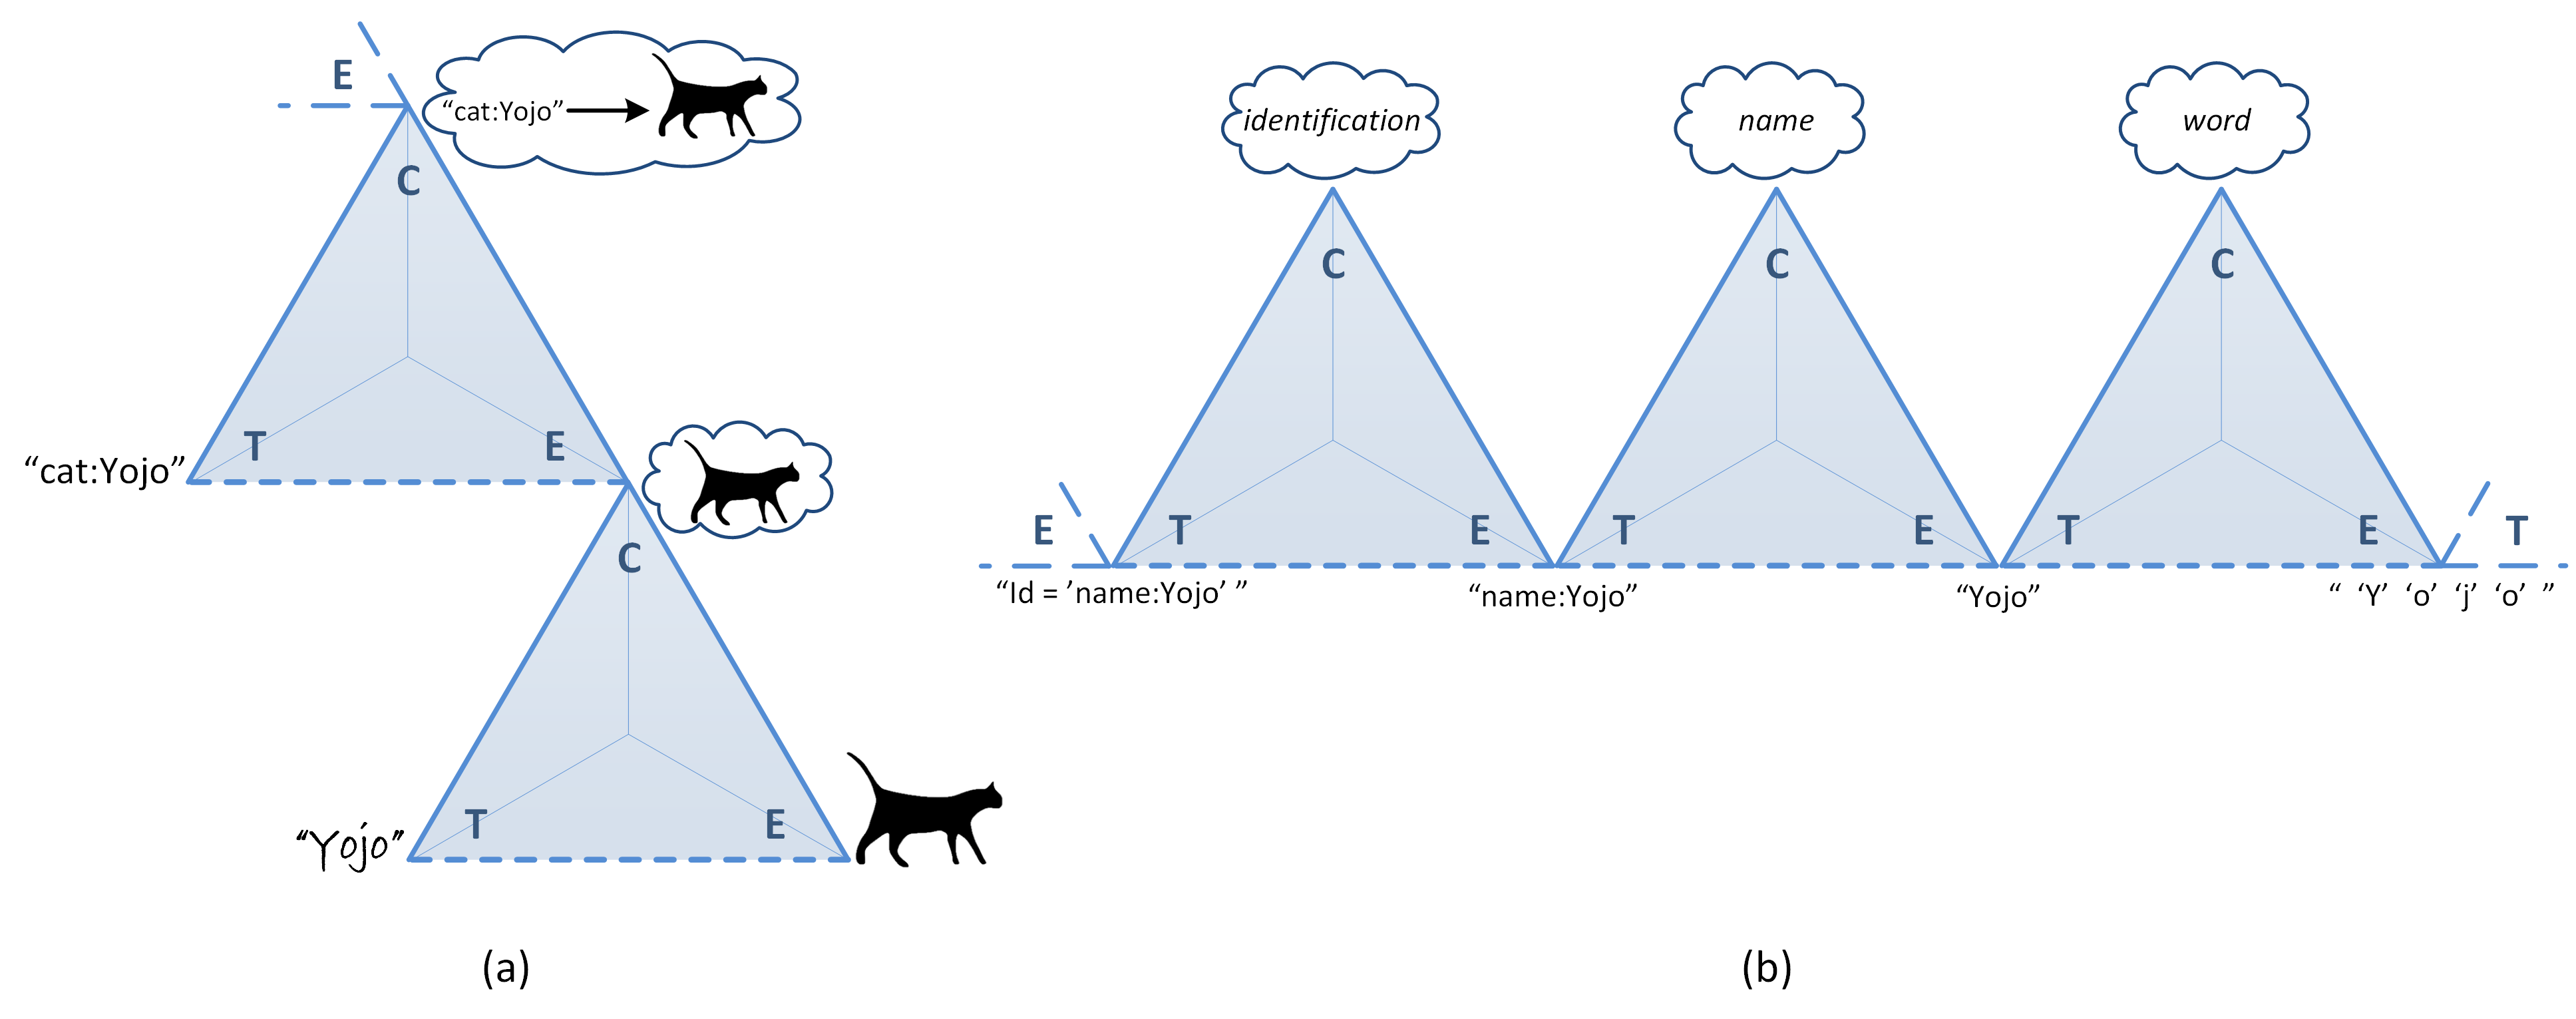
\includegraphics[width=6.25in,height=2.39583in]{./tex2pdf.9980/af5254be7878f6046c2696d66fee3e171cdfcba8.png}
\caption{Linking triadic models together.}\label{fig:linked-triangles}
}
\end{figure}

Peirce also recognised that multiple triangles could be linked together
in various ways (in: Sowa 2000). By stacking them together, as depicted
in \cref{fig:linked-triangles}(a), a conceptualisation is made of
``representing an entity'': the original concept of a \mywordbox{cat}
named ``Yojo'', depicted in \cref{fig:semiotic-triangles}(c), is being
conceptualised as the concept of a \mywordbox{cat named “Yojo”} and
represented by \mywordbox{cat:Yojo}. In (Eco 1976), Eco uses the term
\emph{unlimited semeiosis} to refer to the succession of stacking signs
that emerge from that, ad infinitum. We consider unlimited semeiosis as
addressing a dimension of comprehension about abstraction and
generalisation, with an eventual finish in the ultimate
\mywordbox{Thing} concept. Linking the triangles horizontally results in
different representational metalevels, depicted in
\cref{fig:linked-triangles}(b): From right to left, the characters ``Y''
``o'' ``j'' and ``o'' are conceptualised as a single \mywordbox{word}
and represented as ``Yojo'', which is conceptualised as a
\mywordbox{name} and represented as ``name:Yojo'', which is
conceptualised as an \mywordbox{identifier} that might be represented as
``Id='name:Yojo'''.

\hypertarget{bridgehead-semantics}{%
\chapter{Bridgehead: Semantics}\label{bridgehead-semantics}}

Purpose of this section:

\begin{enumerate}
\def\labelenumi{\arabic{enumi}.}
\tightlist
\item
  From a semiotic perspective, explain what we mean with semantics in
  software agents, i.e., the reciprocity between data and data
  processing code.
\item
  Establish that for representing semantics, descriptive models (i.e.,
  ontologies) trump prescriptive models (all 42010 models).
\item
  Conclude that ontologies need their place as single point of reference
  (trueness) in architectures, and identify their relationship with the
  rest of the architectures, i.e., all other prescriptive models. Note
  the issue on Open World Assumption (ontologies) and CWA (prescriptive
  models).
\end{enumerate}

Argument:

\begin{enumerate}
\def\labelenumi{\arabic{enumi}.}
\item
  Explain shortcomings of 42010:2011 in terms of semiotic triangle:

  \begin{enumerate}
  \def\labelenumii{\arabic{enumii}.}
  \tightlist
  \item
    All models are representations of engineers' conceptualisations
  \item
    In MDA, ``models represent reality'' makes the semiotic triangle
    conflate in a \mywordbox{model}
    \textless{}---\mywordbox{representation}---\textgreater{}
    \mywordbox{reality} dimension,
  \item
    This cuts-off the conceptualisation vertex and with that our
    ``knowledge about our given remark or doctrine \emph{says} there
    is''. We have removed the ``ontological level'' (Guarino 1994), and
    with that, the fact that ``terminological competence can be gained
    by formally expressing the ontological commitment of a knowledge
    base'' (ibid.)
  \item
    (Meta-)model instantiation, and hence level transition, therefore
    remains at the Term/Model vertex
  \item
    The CIM models both semantics (Domain Model) and pragmatics
    (Business Model)
  \item
    Models are ultimately expressed as either Data or Code, both located
    at the Term/Model vertex.
  \item
    The trueness of prescriptive models, i.e., all 42010:2011 models, is
    established against their meta-models, while the trueness of
    descriptive models, i.e., ontologies, is established through the
    interpretation in the conceptualisation of reality (sets and set
    theory)
  \end{enumerate}
\item
  The reciprocity between code and data manifests itself as software
  semantics

  \begin{enumerate}
  \def\labelenumii{\arabic{enumii}.}
  \tightlist
  \item
    The relationship between Data and Code is very closely coupled in
    order to maintain consistency between each other. Inconsistency
    results in software malfunction / crashes. Maintaining/controlling
    that consistency is one of the main goals of MDA/MDE.
  \item
    Inconsistency between Code and Data has either pragmatic grounds
    (i.e., code assumes different reality than data resulting in
    incorrect operations on the data) or semantic grounds (i.e., data
    assumes different reality than the code resulting in incorrect data
    being correctly operated on).
  \end{enumerate}
\item
\end{enumerate}

\hypertarget{what-is-software-semantics}{%
\section{What is software semantics}\label{what-is-software-semantics}}

We take the position that strong AI is not yet available, if ever
(Xiuquan Li and Tao Zhang 2017), and conclude that weak AI is
essentially a token-based machine without the ability to close the gap
between token and reality. Also called the Grounding Problem (Harnad
1990), addressing this fundamental distinction in software engineering
about semantics is at best extremely narrow (Steels 2012), or not
present at all (Cregan 2007). This implies that the semiotic triangle is
denied its conceptualisation vertex, and the sign remains incomplete.
This is confirmed by the software engineering discipline herself
implicitly, since it consistently speaks of `models that represent
reality' without factoring the conceptualisation into the equation,
e.g., ``\emph{a model is a representation of reality intended for some
definite purpose}'' and similar quotes that are collected by (Aßmann et
al. 2006). Consequently, the edges that connect the conceptualisation
remain vague or necessarily conflate on the relationship between the
model and reality, depicted in \cref{fig:software-models-reality}. This
beheaded sign cuts-off our ``knowledge about our given remark or
doctrine \emph{says} there is''. We have removed the ``ontological
level'' (Guarino 1994), and with that, the fact that ``terminological
competence can be gained by formally expressing the ontological
commitment of a knowledge base'' (ibid.). Since we make do with weak AI
and its beheaded sign necessarily, this suggests that genuine semantics
can not ever exist in current software agents.

\begin{figure}
\hypertarget{fig:software-models-reality}{%
\centering
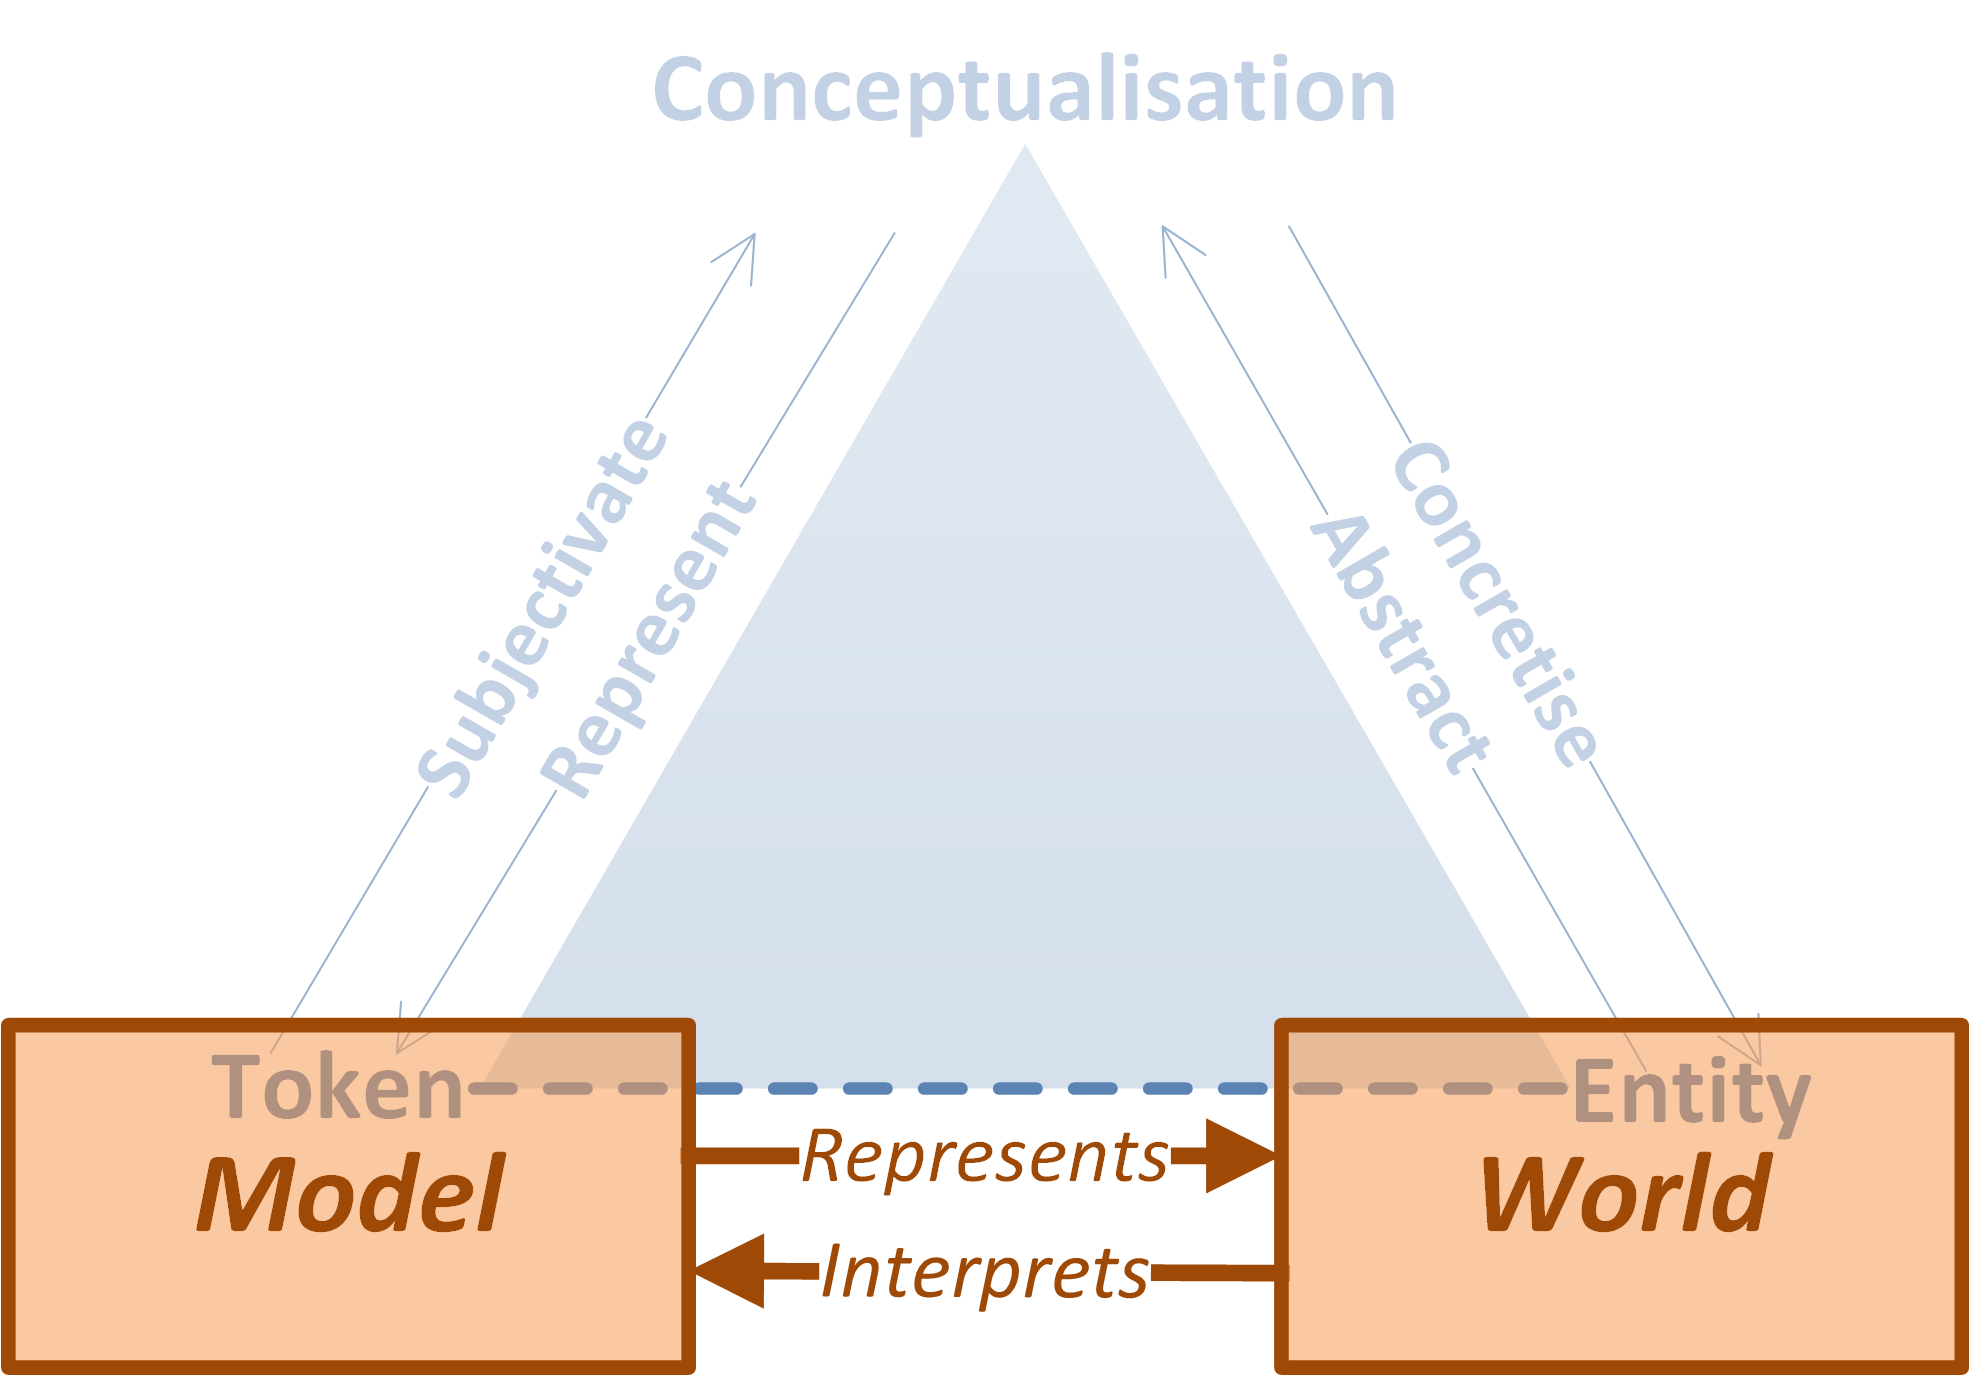
\includegraphics{./tex2pdf.9980/a8961801a1f02a208deeb0559c89c4f1e2bb6725.png}
\caption{Software engineering applies a beheaded semiotic triangle in
which its edges remain vague or conflate in the single relation between
model and reality.}\label{fig:software-models-reality}
}
\end{figure}

During the use of a software agent the semeiosis is taken care of by the
human-in-the-loop, viz. the end user at the human-machine interface
(HMI) whom interprets the tokens that are displayed (subjectivation).
During development of a software agent the semeiosis is taken care of by
another human-in-the-loop, viz. the software engineer whom implicitly
performs the conceptualisation and explicitly represents this
conceptualisation into tokens, i.e., \emph{models}. Consequently, all
models are representations of engineers' conceptualisations. From the
many models that software engineering typically generates we focus on a
pair of models: the information or data models that refer to the
\emph{information entities} in reality, paired with the process or
business models that represent the \emph{event entities} that operate on
the information entities. At this modelling level, semantics still exist
by virtue of the designer. However, when the software agent is
subsequently compiled, its binary code originate from the process model
of the model pair (operations, algorithms), and the memory allocation
for the data originates from the information model of the model pair
(size, format, encoding). At this binary level the software engineer has
left the building, and with him the conceptualisation vertex and the
subsequent capability for semeiosis and, thus, semantics. In other
words, at binary level we have lost the capability to verify the
semantic coherence between the code and the data while the reciprocity
between data and software code determines the semantic validity of the
data processing. For instance, consider a data element \(t\) to
represent temperature, and an algorithm to establish fever, e.g.,
\texttt{t\ \textgreater{}\ 37.0} \(\to\) \texttt{fever}. The one and
only means to keep the software from failing is that both the data and
the algorithm (i) are expressed in the same unit of dimension
(\(\si{\degree}C\) in this example), apply the same (ii) resolution and
(iii) accuracy, to name a few obvious constraints. We, therefore, take
the stance that semantics can only exist in software by virtue of the
semeiosis by the human-in-the-loop, while in the software agent itself
semantics are necessarily reduced to the reciprocity between data and
software code. Still, the software agent acts as transport medium for
the semantics as intended by the software engineer to the semantics as
experienced by the end user at the HMI. We therefore consider the
coherence between the pair(s) of data and data processing models
essential for enforcing the software agent to maintain a semantic valid
reciprocity between binary code and the data it operates on. This leads
to the definition of a (normative (Greefhorst and Proper 2011)) design
principle to its effect:

\begin{mmdp}[Coherence principle]\label{dp:coherence-principle}

\textbf{Essence of principle:} Establish explicit coherence between the model(s) that refer to the information entities in reality and the model(s) that operate on them.

\textbf{Type of information:} business

\textbf{Quality attributes:} (semantic) accuracy, reusability, manageability, understandability 

\textbf{Rationale:}
\begin{itemize}
\item Semantics in software agents are necessarily reduced to, and emerge from, the reciprocity between the data and the binary code that operates on them;  
\item Without explicitly addressing -- at modelling level -- \textbf{all} facets that influence the coherence between the data on the one hand, and the operations that apply on them on the other, the software agent cannot guarantee to maintain the reciprocity between them at the binary level;
\item Without maintaining the reciprocity between binary code and the data it operates on, the semeiosis performed by the end user on the result of the data processing and their subsequent semantics cannot be guaranteed to be similar as intended by the software engineer.
\end{itemize}
\textbf{Implications:}
\begin{itemize}
\item The coherence principle is a necessary condition for supporting semantic interoperability;
\item The scope of semantic validity \& accuracy is addressed explicitly and can be referred to;
\item Reuse of data often implies reuse of the data processing code, and vice versa. Having established explicit coherence improves the quality of data and code reuse, and facilitates the verification that the scope of the semantic validity \& accuracy applies in the new context as well;
\item manageability ...?
\item understandability ...?
\end{itemize}  
\end{mmdp}

Coherence between models can be established with use of a single unique
reference against which the truth of the expressions of both models can
be verified. In semiotics, this single unique reference is considered
reality, as indicated in \cref{fig:semiotic-triangles}(b) by the
\emph{trueness} characteristic. Except as toy example in (Steels 2012),
this is clearly not possible. The \emph{correctness} characteristic is
the only alternative left, taking the conceptualisation node as its
principle point of reference. This is exactly what the mathematical
branch of \emph{formal semantics} achieves (Gamut 1991; Genesereth and
Nilsson 1987) with its three main characteristics, viz. connecting (i)
an abstract syntax of a language to (ii) a domain of interpretation
(usually a set theoretic framework) by defining (iii) an interpretation
function from the abstract syntax onto the set theoretic framework. In
terms of the semiotic triangle, \cref{fig:semiotic-triangles}(b), this
implies the following:

\begin{enumerate}
\def\labelenumi{(\roman{enumi})}
\tightlist
\item
  the \emph{representation} node represents models that can be
  formulated by use of an abstract syntax (and grammar) as its modelling
  language. In this reading, a model is a particular constellation of
  tokens that represent a particular state of affairs;
\item
  a particular \emph{conceptualisation} can be mathematically formulated
  as a specific constellation of (unnamed) individuals, sets of
  individuals, and sets of sets;
\item
  the \emph{subjectivation} edge can be formulated as the interpretation
  function that assigns a mapping from modelling language tokens onto
  the set elements, enabling the evaluation of a specific model against
  the intended conceptualisation from (i).
\end{enumerate}

Formal semantics thus provides a means to formulate a particular
conceptualisation as principle point of reference to establish the
coherence between two models. In the remainder of this text we will
refer to the formulation of the reference conceptualisation as a
\emph{conceptual model}.

In conclusion, we explain software semantics as the reciprocity between
data and software code, realised by maintaining the coherence between
pairs of data and data processing models, by applying formal semantics
to formulate a particular conceptualisation as semantic reference, and
an interpretation function from the data and operation models to that
reference.

\hypertarget{explicit-semantics}{%
\section{Explicit semantics}\label{explicit-semantics}}

Explicit semantics

This shows how the cognitive quality of the conceptualisation could be
substituted with a formulation in set theory. The resulting conceptual
model essentially remains a representation, albeit a mathematical one.
One can argue that such substitution does not resolve the grounding
problem, and appropriately so. Still, mathematics provides for a very
exact way to express oneself, reducing the ambiguity that comes
implicitly with any other language. Furthermore, logical constructs used
at the syntactical level can be interpreted into set theoretic
operations, facilitating the evaluation of complicated expressions. And
thanks to mathematics we can also indicate the exact issues that exist
with conceptual modelling, depicted in
\cref{fig:4-model-construct-issues}.

{[}Four different types of construction issues that come with formal
semantics{]}{[}def:constructissues{]}

This begs the question what we mean with model, and what criteria we
should adopt to represent a conceptual model.

An appropriate definition for ontology is given by \cite{Guarino:1998wq}
as a ``logical theory accounting for the intended meaning of a formal
vocabulary''.

The triadic model is more suitable to explain the differences between
human semantics and semantics in computers, by identifying the semiotic
differences between the two as follows. Since humans are capable of
making observations from reality, and abstract these into
conceptualisations, there is a direct connection between the entity and
the conceptualisation. Computers lack that capability, as depicted in
\cref{fig:semiotic-differences}. Here, we show the semiotic differences
between semantics as they appear for human actors, part (a) of the
Figure, and that of software actors in part (b). The comparison is made
from the perspective of communication, e.g., how is reality signified
into utterances made by the actor, and vice versa, how are utterances
signified into what they stand for in reality. We can assume the entity
to remain identical over both actors, and the token to remain equivalent
to the extent that in terms of computers these are referred to as
\emph{data}. The third node, representing the conceptualisation for
human agents, for software agents we claim to denote that as the
application. Although in its bare form an application is nothing more
than tokens that follow a specific language grammar, this bare form is
only a representation of its quintessence, i.e., a run-time notion on
how to act on the receipt of data.

However, because computers are unable to conceptualise or concretize,
the connection between the software's conceptualisation and the entity
does not exist. This ``missing link'' in artificial intelligence is
called \emph{the grounding problem}, named after the inability to ground
a conceptualisation in what it refers to in reality. In literature, two
exceptions to this rule exist, which we discuss in the box text below.
Our stance towards these exceptions is that they are interesting,
however currently irrelevant towards the resolution of semantic
interoperability due to their many practical shortcomings in
implementing an actual connection between the entity and the
conceptualisation.

\begin{figure}
\hypertarget{fig:semiotic-diffs}{%
\centering
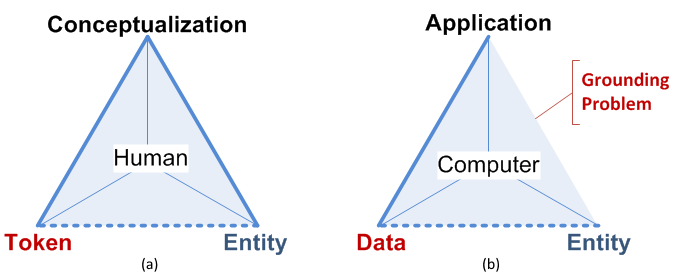
\includegraphics{./tex2pdf.9980/1ce00968991a55f6ab1ac66202d4d01993d7c060.png}
\caption{Semiotic differences in semantics for humans and
computers}\label{fig:semiotic-diffs}
}
\end{figure}

This is known as the \emph{problem of reference}, a manifestation of the
\emph{grounding problem}.

In information systems, addressing the distinction between terms and
reality is extremely limited (Steels 2012), or not present at all
(Cregan 2007).

Artificial intelligence (AI) tries to tackle the grounding problem by
building some form of understanding, also known as ``strong AI''.
However, strong AI is expected to emerge on the long term only, if ever
(Xiuquan Li and Tao Zhang 2017). Its counterpart ``weak AI'',
characterised by logic and reasoning, relies on language only and can
therefore never make the step to reality on its own (Scheider 2012).

Hierin duidelijk maken wat de verschillen zijn tussen modellen en
ontologie. Semiotiek (eigenlijk de semiotische driehoek) gebruiken wij
als methode om te verklaren wat semantiek is bij mensen en bij
computers. En zonder semantiek in de architectuur, geen SIOp.

CONCLUSIE: Architectures will not be able to facilitate semantics and,
hence, consolidate SIOp without including semiotics. Assumption 1: root
cause for SIOp issues is the grounding problem: GP leads to absence of
semantics, absence of semantics leads to absence of SIOp. Fact: Strong
AI could solve GP, but doesn't exist Fact: Weak AI is based on language
only, and can never solve GP on its own Observation: Humans can solve
GP, semiotics explain why Fact: Semiotics studies relation between
language (terms) and meaning

Thus, weak AI is our only option for the time being in order to achieve
semantics and SIOp.

We therefore cannot neglect the existence of the grounding problem and
its semiotic origins. Nevertheless, we do. For instance, when we are
asked to explain how we address the grounding problem in the design of
our software agent, we can't; when we are asked to point at the
semantics parts in the code of our software agent, we can't. The same
question however about, e.g., its scalability, will render a lecture
with adequate references to the underlying architecture. We thus remain
at a loss of how to engineer semantics into software agents. However,
without a clear understanding on semantics and its contribution to the
software agent, we are lacking the bridgehead within the software agent
that is fundamental to the semantic interoperability bridge.

In fact, this is a question of philosophy while ICT is ``only'' faced
with its consequence: computers can deal with language only and have no
clue about reality.

It therefore remains impossible to ground the applied terms in reality,
denoted as the \emph{grounding problem}. Its resolution is a major
subject in strong AI and in (geographic) information science in general
\cite{Scheider:2012tj}. Although \cite{Steels:2008tr} provides for an
alternative (weak AI) solution, that only shows the need to refer to
general stance is that the grounding problem remains a big challenge .

\hypertarget{spanning-alignments}{%
\chapter{Spanning: Alignments}\label{spanning-alignments}}

Purpose of this Section:

\begin{enumerate}
\def\labelenumi{\arabic{enumi}.}
\item
  Determine that data exchange inevitably breaks the necessary atomic
  semantic monolith between data and data processing code.
\item
  Follow the coherence principle and conclude that the models from which
  \emph{external} data and \emph{receiving} data processing code are
  derived, need to be brought into coherence with each other.
\item
\end{enumerate}

\begin{center}\rule{0.5\linewidth}{\linethickness}\end{center}

despite the notoriously difficult philosophical questions involved,
semantic interoperability can be seen as an engineering problem, namely
that of effectively constraining interpretations towards the ones that
are considered allowable.

\begin{figure}
\hypertarget{fig:2semiotic-triangles}{%
\centering
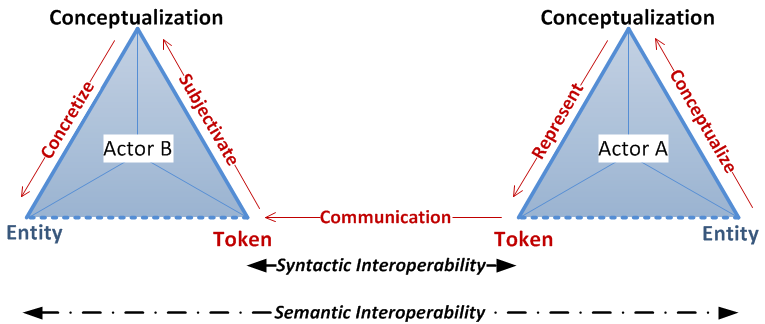
\includegraphics[width=0.9\textwidth,height=\textheight]{./tex2pdf.9980/fac83dcaa0ef39be01bcba4da966101b9332f127.png}
\caption{The various forms of
interoperability}\label{fig:2semiotic-triangles}
}
\end{figure}

\hypertarget{references}{%
\chapter*{References}\label{references}}
\addcontentsline{toc}{chapter}{References}

\setlength{\parindent}{-0.2in}

\setlength{\leftskip}{0.2in}

\setlength{\parskip}{8pt}

\hypertarget{refs}{}
\leavevmode\hypertarget{ref-Auxdfmann2006}{}%
Aßmann U, Zschaler S, Wagner G. 2006. Ontologies, Meta-models, and the
Model-Driven Paradigm. In \emph{Ontol. Softw. Eng. Softw. Technol.} (C.
Calero, F. Ruiz, and M. Piattinieds. ), pp. 249--273, Springer-Verlag
Berlin Heidelberg.

\leavevmode\hypertarget{ref-Cregan2007}{}%
Cregan AM. 2007. Symbol grounding for the semantic web. W. Franconi, E
and Kifer, M and Mayed.. Semant. WEB res. Appl. Proc. 4519: 429--442.

\leavevmode\hypertarget{ref-Eco1976}{}%
Eco U. 1976. \emph{A theory of semiotics}. Indiana University Press /
London: Macmillam, Bloomington, IN.

\leavevmode\hypertarget{ref-Gamut1991}{}%
Gamut L. 1991. \emph{Logic, Language and Meaning, volume 1: Introduction
to Logic}. The University of Chicago Press.

\leavevmode\hypertarget{ref-Genesereth:1987dg}{}%
Genesereth MR, Nilsson NJ. 1987. \emph{Logical foundations of artificial
intelligence}. Morgan Kaufmann Publishers Inc.

\leavevmode\hypertarget{ref-Greefhorst2011}{}%
Greefhorst D, Proper E. 2011. \emph{Architecture Principles, The
Cornerstones of Enterprise Architecture}. Springer Berlin Heidelberg.

\leavevmode\hypertarget{ref-Guarino1994b}{}%
Guarino N. 1994. The Ontological Level. R. Casati, B. Smith, and G.
Whiteeds. Philos. Cogn. Sci. Proc. 16th int. Wittgenstein symp.
443--456;
doi:\href{https://doi.org/10.1007/978-3-642-02463-4}{10.1007/978-3-642-02463-4}.

\leavevmode\hypertarget{ref-Harnad1990}{}%
Harnad S. 1990. The Symbol Grounding Problem. Physica D 42. 335--346.

\leavevmode\hypertarget{ref-Ogden1989}{}%
Ogden CK, Richards IA. 1989. \emph{The Meaning of Meaning: A Study of
the Influence of Language upon Thought and of the Science of Symbolism}.
with a pre. Harcourt Brace Jovanovich, New York, USA.

\leavevmode\hypertarget{ref-Saussure:1983ka}{}%
Saussure F de. 1959. \emph{Course in general linguistics}. C. Bally and
A. Sechehayeeds.. Philosophical Library, New York, USA.

\leavevmode\hypertarget{ref-Scheider:2012tj}{}%
Scheider S. 2012. Grounding geographic information in perceptual
operations. Dissertation, Westfälische Wilhelms-Universität Münster; IOS
Press.

\leavevmode\hypertarget{ref-Searle:1980hw}{}%
Searle JR. 1980. Minds, brains, and programs. Behav. Brain Sci. 3:
417--424.

\leavevmode\hypertarget{ref-Sowa:2000di}{}%
Sowa JF. 2000. Ontology, metadata, and semiotics. Lect. Notes Comput.
Sci. (including Subser. Lect. Notes Artif. Intell. Lect. Notes
Bioinformatics) 1867:55--81;
doi:\href{https://doi.org/10.1007/10722280_5}{10.1007/10722280\_5}.

\leavevmode\hypertarget{ref-Steels:2008tr}{}%
Steels L. 2012. The symbol grounding problem has been solved, so what's
next. In \emph{Symb. Embodiment debates mean. Cogn.} (M. de Vega, A.
Glenberg, and A. Graessereds. ), pp. 223--244, Oxford University Press,
Oxford, UK.

\leavevmode\hypertarget{ref-Ullmann:1979sL}{}%
Ullmann S. 1962. \emph{Semantics: An Introduction to the Science of
Meaning}. 1st ed. Basil Blackwell, Oxford.

\leavevmode\hypertarget{ref-XiuquanLi2017}{}%
Xiuquan Li, Tao Zhang. 2017. An exploration on artificial intelligence
application: From security, privacy and ethic perspective. J. Zhu, E.-B.
Lin, and T. Lieds. 2017 ieee 2nd int. Conf. Cloud comput. Big data anal.
416--420;
doi:\href{https://doi.org/10.1109/ICCCBDA.2017.7951949}{10.1109/ICCCBDA.2017.7951949}.

%\chapter*{References}
% --- index --- --- --- --- ---


\printindex

%ACKNOWLEDGMENTS are optional
%\chapter*{Acknowledgments}
% % 
\end{document}
